\documentclass[12pt]{article}
\usepackage[left=2cm,right=2cm,top=2cm,bottom=2cm]{geometry}
\usepackage{wrapfig}
\usepackage{booktabs}
\usepackage{graphicx}
\usepackage{amssymb}
\usepackage{siunitx} % Required for alignment
\usepackage{subfigure}
\usepackage{multirow}
\usepackage{rotating}
\usepackage[T2A]{fontenc}
\usepackage[russian]{babel}
\usepackage{caption}
\usepackage{hyperref}
\usepackage{mathtools}
\usepackage{amsmath}
\usepackage{float}
\usepackage{mathrsfs}

\hypersetup{
    colorlinks=true,
    linkcolor=blue,
    urlcolor=magenta,
    citecolor=cyan,
    }
\graphicspath{{pictures/}}

\begin{document}
  \begin{titlepage}
      \begin{center}
          \vspace*{1cm}

          \Huge
          \textbf{ЭФФЕКТ ЗЕЕМАНА}

          \vspace{1.5cm}

          \Large
          \textbf{Балдин Виктор Б01-303\\
                  Рачинский Максим Б01-303}

          \vfill

          Вопрос по выбору \\
          Устный экзамен по общей физике

          \vspace{0.8cm}

          
\includegraphics[width=0.4\textwidth]{university_logo.png}

          Физтех-школа радиотехники и компьютерных технологий\\
          Московский физико-технический институт\\
          Долгопрудный, 2025
      \end{center}
  \end{titlepage}

  \tableofcontents

  \section{Введение}
  В 1896 г. Зееман (1865-1943) обнаружил, что спектральные линии определенным образом расщепляются, если источник света поместить в магнитное поле. В опыте Зеемана исследовалась очень узкая зелено-голубая линия кадмия и применялись магнитные поля с напряженностью $10000-15000$ Гс. Г.А. Лорентц, развивавший в то время электронную теорию, сразу же объяснил явление Зеемана и тем самым придал дальнейшим исследованиям планомерный и целенаправленный характер.

  Применяемая схема для наблюдения и исследования явления приведена на рис. \ref{fig:scheme}. Источник света с линейчатым спектром (например, газоразрядная трубка или вакуумная дуга) помещается между полюсами электромагнита, создающего достаточно однородное магнитное поле. Исследуемый свет попадает на щель

  \begin{figure}[H]
    \centering
    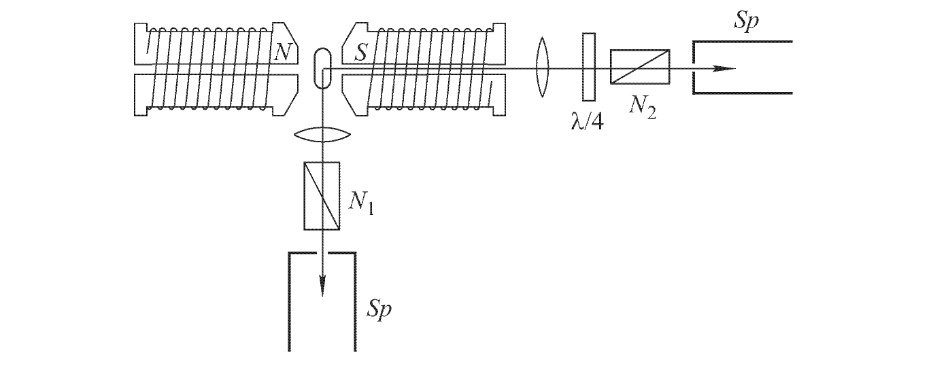
\includegraphics[width=\textwidth]{scheme.png}
    \caption{Схема для наблюдения}
    \label{fig:scheme}
  \end{figure}
  спектроскопа или спектрографа $S p$ с разрешающей силой около 100000 или выше (дифракционную решетку или интерференционный спектральный аппарат). Николи $N_1, N_2$ и пластинка $\lambda / 4$ служат для исследования поляризации излучаемого света. При фотографировании наблодаемой картины применяются иногда многочасовые экспозиции. В течение всего этого времени должно быть обеспечено с достаточной точностью постоянство магнитного поля и температуры источника, чтобы картина оставалась неизменной во времени и можно было использовать спектральный аппарат высокой разрешающей силы.

  В первых опытах Зееман обнаружил, что при наблюдении поперек поля спектральная линия расщепляется на три линейно поляризованные компоненты. Средняя компонента не смещена, крайние смещены в противоположные стороны на одинаковые расстояния (в шкале частот). Смещение пропорцнонально напряженности внешнего магнитного поля В. В средней компоненте электрический вектор направлен параллельно магнитному полю (такие компоненты называются $\pi$-компонентами), в крайних - перпендикулярно к нему (такие компоненты называются $\sigma$-компонентами). Интенсивность $\pi$-компоненты в,двое, а каждой пз $\sigma$-компонент в четыре раза меньше интенсивности исходной линии.

  При наблюдении вдоль маглитного поля получается такое же смещение (прн одинаковой напряженности магнитного поля), что и в предыдущем случае, но несмещенная компонента отсутствует. Интенсивность каждой компоненты в,двое меньше интенсивности исходной спектральной линии. Обе компоненты поляризованы по кругу в противоположных направлениях (их принято называть также $\sigma$-комнонентами). Если свет распространяется в направлении магнитного поля, то $\sigma$-компонента с меньшей частотой поляризована по правому, а с большей - по левому кругу. При изменении направления магнитного поля на противоположное меняется на противоположную и крутовая поляризация обеих компонент.

  \begin{wrapfigure}{l}{0.5\textwidth}
    \centering
    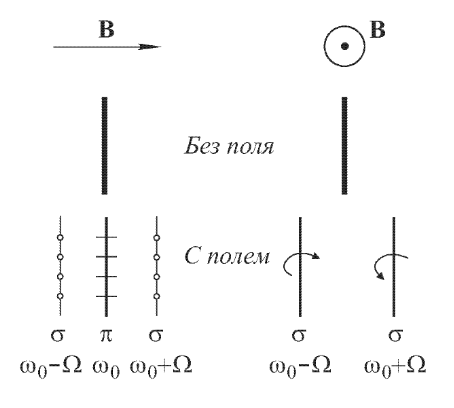
\includegraphics[]{pole.png}
    \caption{}
    \label{fig:pole}
  \end{wrapfigure}

  Картина, наблюдаемая поперек и вдоль магнитного поля, представлена схематически на рис. \ref{fig:pole}. Преднолагается, что в случае продольного эффекта свет распространяется вдоль магнитного поля, направленного к чнтателю. Относительные интенсивности линий показаны их толщиной, поляризация $\pi$-компоненты - штрихами, параллельными магнитному полю, а $\sigma$-компонент - кружочками.

  \section{Теория Лорентца}
  Описанная картина расщепления спектральных линий объясняется классической теорией Лорентца. Как и классическая теория дисперсии, это есть модельная теория, в простейшей форме которой излучающими центрами являются гармонические осцилляторы в виде квазиупруго связанных электронов. В отсутствие внешнего магнитного поля уравнение движения такого электрона имеет вид $\ddot{\mathbf{r}}+\omega_0^2 \mathbf{r}=0$, где $\omega_0$ - собственная частота электрона. При наличии постоянного магнитного поля на электрон действует еще сила Лорентца $-\frac{e}{c}[\dot{\mathbf{r B}}]$ (заряд электрона обозначен через $-e$ ). Уравнение движения электрона принимает вид

  \[
  \ddot{\mathbf{r}}+\omega_0^2 \mathbf{r}=-\frac{c}{m c}[\dot{\mathbf{r}} \mathbf{B}],
  \]


  где $m$ - масса электрона. Введя ларморовскую частоту

  \begin{equation}
  \boldsymbol{\Omega}=\frac{c}{2 m c} \mathbf{B},
  \label{eq:larm}
  \end{equation}


  приведем его к виду

  \begin{equation}
  \ddot{\mathbf{r}}+2[\dot{\mathbf{r}} \boldsymbol{\Omega}]+\omega_0^2 \mathbf{r}=0
  \label{eq:center}
  \end{equation}

  (см. \cite[\S 86]{sivykhin3}). Классическая теория сводится к решению этого уравнения. Для решения уравнения (\ref{eq:center}) перейдем к координатной форме. Направим ось $Z$ прямоутольной системы координат влоль магнитного поля В. Тогда предыдущее уравнение сведётся к системе трёх скалярных уравнений
  \begin{equation}
  \begin{cases}
  \ddot{x} + 2\Omega \dot{y} + \omega_0^2 x = 0 \\
  \ddot{y} - 2\Omega \dot{x} + \omega_0^2 y = 0 \\
  \ddot{z} + \omega_0^2 z = 0.
  \end{cases}\,.
  \label{eq:coord}
  \end{equation}

  Из последнего уравнения видно, что магнитное поле не влияет на движение электрона вдоль магнитного поля. Это и понятно, так как при таком движении не возникает силы, действующей со стороны магнитного поля. Интегрирование первых двух уравнений (\ref{eq:coord}) удобно провести в комплексной форме. Объединим $x$ и $y$ в комплексную координату $\zeta = x + iy$. Она определяет положение электрона в координатной плоскости $(X, Y)$ совершенно так же, как это делается с помощью двумерного вектора с составляющими $x$ и $y$. Заметив, что $-i\dot{\zeta} = \dot{y} - i\dot{x}$, умножим второе уравнение (\ref{eq:coord}) на $i$ и сложим с первым. Тогда
  \[
  \ddot{\zeta} - i \cdot 2\Omega \dot{\zeta} + \omega_0^2 \zeta = 0.
  \]

  Ищем решение этого уравнения в виде $\zeta = e^{i\omega t}$. Постоянная $\omega$ найдётся из квадратного уравнения
  \[
  -\omega^2 + 2\Omega \omega + \omega_0^2 = 0,
  \]
  которое даёт
  \[
  \omega = \Omega \pm \sqrt{\omega_0^2 + \Omega^2}.
  \]

  \begin{wrapfigure}{r}{0.5\textwidth}
    \centering
    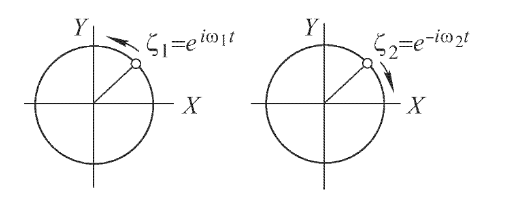
\includegraphics[]{circle.png}
    \caption{}
    \label{fig:circle}
  \end{wrapfigure}

  Даже в очень сильных магнитных полях квадратом ларморовской частоты можно пренебречь по сравнению с $\omega_0^2$. Например, если $B = 10^4$ Гс, то формула (\ref{eq:larm}) даёт $\Omega \approx 10^{11}~\text{с}^{-1}$, тогда как для видимого света ($\lambda = 500$ нм) $\omega \sim 4 \cdot 10^{15}~\text{с}^{-1}$, а потому $(\Omega/\omega)^2 \sim 10^{-9}$. Максимальное магнитное поле, в котором измерялось земнокосмическое расщепление спектральной линии, получено в 1938 г. П.П. Капицей (1894–1984). Оно было $3.2 \cdot 10^5$ Гс. Даже в этом случае $(\Omega/\omega)^2 \sim 1.4 \cdot 10^{-3}, (\Omega/\omega)^2 \sim 2 \cdot 10^{-6}$. Таким образом, с большой точностью $\omega = \pm \omega_0 \pm \Omega$. Чтобы не пользоваться отрицательными частотами, введём переобозначение, положив $\omega_1 = \omega_0 + \Omega, \omega_2 = \omega_0 - \Omega$. Тогда полученные ранее решения запишутся в виде
  \[
  \zeta_1 = e^{i\omega_1 t}, \quad \zeta_2 = e^{-i\omega_2 t}.
  \]

  Первое решение представляет круговое движение, в котором электрон вращается против часовой стрелки с угловой частотой $\omega_1$, второе — также круговое движение, но по часовой стрелке и с частотой $\omega_2$ (рис. \ref{fig:circle}). Общее решение соответствует наложению таких двух вращений и представляется в виде $\zeta = C_1 \zeta_1 + C_2 \zeta_2$, где $C_1$ и $C_2$ — произвольные постоянные.

  Чтобы нагляднее увидеть полученные результаты, разложим первоначальное движение электрона (т.е. движение в отсутствие магнитного поля) на прямолинейное колебание в направлении оси $Z$ и на движение в плоскости $XY$. Второе движение в отсутствие поля разложим на два круговых вращения с одной и той же угловой частотой $\omega_0$, но совершающихся в противоположных направлениях. При включении магнитного поля колебание вдоль оси $Z$ остаётся неизменным. Частоты же обоих вращений изменяются на одну и ту же величину $\Omega$: если вращение совершается против часовой стрелки, то частота увеличивается, а если по часовой стрелке, то уменьшается.

  Для изменения частоты при вращении по кругу можно привести простое объяснение. Центростремительная сила, действующая на вращающийся электрон в отсутствие магнитного поля, равна $m_0 \omega_0^2 r$. В магнитном поле к ней добавляется сила $\pm \frac{e}{c} v B = \pm \frac{e}{c} \omega r B$, так что новая центростремительная сила становится равной
  \[
  m_0 \omega^2 r \pm \frac{e}{c} \omega B = m_0 (\omega_0^2 \pm 2\Omega \omega).
  \]

  Выбор знака зависит от направления вращения. Приравняв это выражение $m_0 \omega^2 r$, приходим к уравнению $\omega^2 = \omega_0^2 \pm 2\Omega \omega$, из которого для положительных корней находим $\omega = \omega_0 \pm \Omega$. Это совпадает с результатами, полученными выше.

  При включении магнитного поля кинетическая энергия вращения электрона изменяется. Возникает вопрос, как это может происходить, если сила, действующая со стороны магнитного поля, перпендикулярна к скорости и, следовательно, работы не совершает? Ответ состоит в том, что последнее утверждение относится к \textit{установившимся магнитным полям}, которые только и учитываются уравнением (\ref{eq:center}). Но при включении магнитного поля оно изменяется во времени от нуля до максимального значения, а в дальнейшем либо вообще не включается, либо остаётся постоянным. Во время же нарастания магнитного поля, согласно закону индукции Фарадея, возбуждается \textit{индукционное электрическое поле}, которое совершает работу над электроном, меняя его кинетическую энергию. Когда магнитное поле становится постоянным, кинетическая энергия уже полна и дальнейшее изменение кинетической энергии вращения электрона прекращается, пока не будет вновь включено магнитное поле. В этом установившемся варианте и относятся движения, изображённые выше. Подробное рассмотрение механизма изменения кинетической энергии вращения электрона было приведено в
  \cite[\S 88]{sivykhin3}.

  \section{Расщепление спектра в магнитном поле}
  Перейдём теперь к объяснению расщепления спектральных линий в магнитном поле. Возбуждённый электрон излучает электромагнитные волны. Излучение максимально в направлении, перпендикулярном к движению электрона, а в направлении ускорения отсутствует. Согласно классической теории, частота излучения света совпадает с частотой колебаний электрона. Но последняя меняется при включении магнитного поля. Поэтому должна измениться и частота излучаемого света. При наблюдении вдоль магнитного поля колебание в том же направлении излучения не имеет. Излучение создаётся \textit{только круговыми вращениями электрона}. В результате наблюдаются две $\sigma$-компоненты с круговой поляризацией и частотами $\omega_0 + \Omega$ и $\omega_0 - \Omega$. Если свет идёт в направлении вектора $\mathbf{B}$, то поляризация первой линии будет \textit{левой}, а второй — \textit{правой}. При изменении направления магнитного поля на противоположное меняется направление поляризации круговых колебаний, каждой линии. При наблюдении поперёк магнитного поля B колебания электрона, дающие излучение B, дают максимум излучения. Им соответствует \textit{немеселённая $\pi$-компонента}, в которой электрический вектор параллелен $\mathbf{B}$. Оба круговых движения совершаются в плоскости, перпендикулярной к $\mathbf{B}$. Разложим каждое из них на гармоническое колебание вдоль линии наблюдения и перпендикулярное к нему. Только колебания, перпендикулярные к линии наблюдения, сопровождаются излучением и дают две $\sigma$-компоненты с частотами $\omega_0 + \Omega$ и $\omega_0 - \Omega$, в которых электрическое поле \textit{перпендикулярно} к $\mathbf{B}$.

  Таково объяснение расщепления спектральных линий, наблюдавшегося в первых опытах Зеемана. Если учесть, что в отсутствии магнитного поля все направления движения электрона равновероятны, то нетрудно объяснить и относительные интенсивности спектральных линий в этих опытах.

  Как и из численного примера, приведённого выше ($B = 10^4$ Гс), $(\Omega/\omega)^2 \sim 2 \cdot 10^{-5}$. Для практических этого расщепления требуется спектральное приборы с разрешающей силой $\omega_0 / \Omega$ не менее $5 \cdot 10^4$, т.е. дифракционные решётки или интерференционные спектроскопы. В опытах П.Л. Капицы ($B = 3.2 \cdot 10^5$ Гс) были уже достаточно призменные спектроскопы.

  Исследуя характер круговой поляризации линий в продолженном эффекте Зеемана, можно определить \textit{знак заряда}, вызывающего этот эффект. Он оказался \textit{отрицательным}. Измеряя же величину расщепления, можно определить удельный заряд $e/m$. Он оказался таким же, как и при измерениях по отклонениям катодных лучей в электрических и магнитных полях
  ($e/m = 1{,}759 \cdot 10^7$ СГСМ). Это не оставляет сомнений в том, что заряженные частицы, определяющие оптическое поведение атомов, действительно являются \textit{электронами}.

  \section{Мультиплеты}
  Дальнейшие опыты показали, что явление Зеемана в том виде, в каком оно наблюдалось сначала и нашло объяснение в теории Лоренца — \textit{лонгитюдный эффект}, состоящий из одной $\pi$-компоненты и двух $\sigma$-компонент, а также дублет из двух $\sigma$-компонент, поляризованных по кругу, — наблюдается крайне редко. Такое расщепление называется \textit{нормальным} или \textit{простым эффектом Зеемана}. Подобный эффект почти так же мал, как явление синхротронное, т.е. одиночные, практически монохроматические спектральные линии. Подавляющее большинство спектральных линий являются \textit{мультиплетами} (дублетами, триплетами, квартетами и т.д.), т.е. состоят из нескольких тесно расположенных спектральных линий.

  Простейшим примером мультиплета (дублета) может служить двойная $D$-линия натрия. Она состоит из двух близко расположенных линий с длинами волн $\lambda_1 = 589{,}5930$ нм и $\lambda_2 = 588{,}99693$ нм, причём интенсивность линии $D_2$ вдвое больше интенсивности линии $D_1$.

  Мультиплеты в магнитных полях дают значительно более сложную картину расщепления, чем расщепление в простом эффекте Зеемана. Так, линия $D_1$ натрия расщепляется на \textit{четыре линии}: средние из них являются $\pi$-, а крайние — $\sigma$-компонентами. Линия же $D_2$ расщепляется на \textit{шесть компонентов}: две средние — $\pi$-, а четыре крайние — $\sigma$-компоненты. Таким образом, весь дублет расщепляется на 10 линий. Наблюдаются и более сложные случаи расщеплений мультиплетов. Такие расщепления называются \textit{аномальным или сложным эффектом Зеемана}. Однако этот термин ``сложный эффект'' является неправильным, а не просто эффект \textit{является правилом, а не исключением}.

  Объяснение сложного эффекта Зеемана дала квантовая теория, и на то после того, как был открыт \textit{спин} (т.е. собственный момент количества движения) и связанный с ним \textit{магнитный момент электрона}. В случае симметричных спектральных линий квантовая теория приводит к тем же результатам, что и простая теория Лоренца.


  \bibliography{references}
  \bibliographystyle{gost}

\end{document}
